\chapter{Results}\label{chp:chapter4}
\section{Survey Responses}
As discussed previously, a participation rate of 35-48\% was necessary for a 10\% sampling error and 80\% confidence level. This allowed for inferences to be made on the population, not just the students sampled. The CS and IS senior classes were estimated by their respective departments to be one hundred students each, so participation from twenty-one students was necessary for each major. The IT senior class was estimated at forty students, requiring participation from sixteen students. Table~\ref{tab:response-rates} shows the amount of responses received compared to the total amounts needed.

\begin{table}[h!]
  \centering
  \caption{Response Rates of Various Majors}
  \label{tab:response-rates}
  \begin{tabular}{llllll}
    \toprule
    Major & Total seniors in major & Surveys needed & Surveys received & Response rate\\
    \midrule
    CS    & 100                    & 35             & 40               & 40\%\\
    IS    & 100                    & 35             & 2                & 2\%\\
    IT    & 40                     & 14             & 22               & 55\%\\
    \bottomrule
  \end{tabular}
\end{table}

There were many complications getting responses from IS students. IS seniors do not have a capstone or senior seminar class, so there was no common opportunity to reach them. Since the Learning Style Inventory (LSI) is copyrighted and licensed for hardcopy use, it couldn't be digitized for distribution. This made it difficult to get surveys into the hands of the IS students. After trying for a year to get surveys out and being stonewalled by significant distribution problems, only two surveys from IS students were completed, and those were only completed because those students were in an IT course in which the surveys were distributed. No additional surveys were returned from IS students.

Because of the complications surrounding the IS responses, the IS results were not included in the analysis.

\section{What the LSI Responses Mean}
A student's learning preference on the two axes of the LSI can be seen in Figure~\ref{fig:learning-preferences} which shows the cognitive preferences throughout the LSI spectrum. These preferences can be either in abstract conceptualization (AC), active experimentation (AE), concrete experience (CE), reflective observation (RO), or along the AC$-$CE or AE$-$RO spectrums.

\begin{figure}[h!]
  \centering
  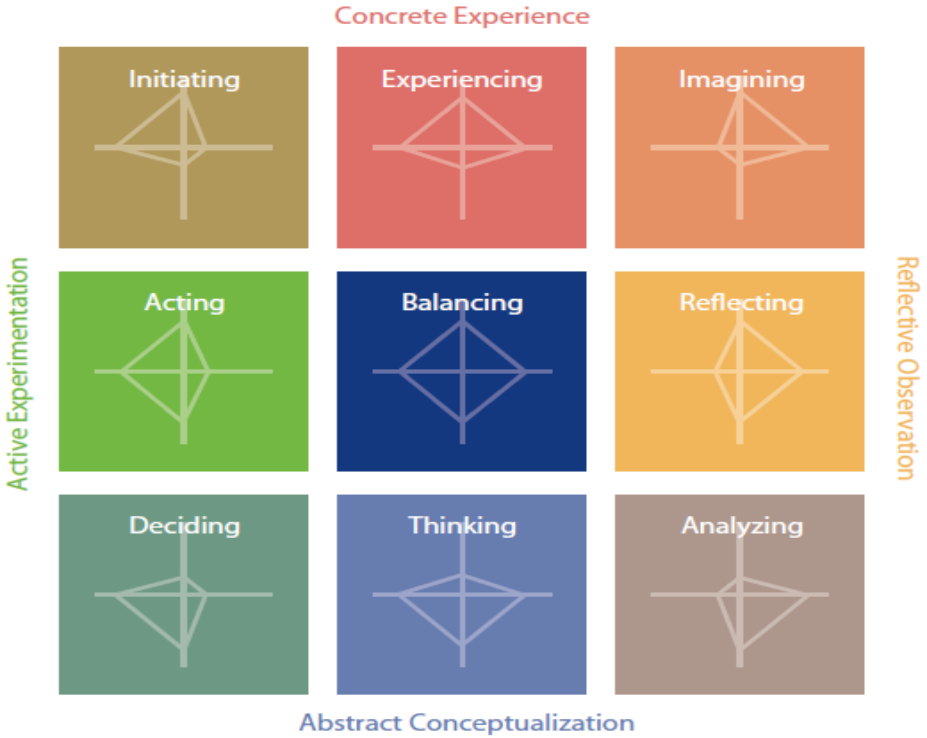
\includegraphics[width=0.9\textwidth]{figures/chapter4/learning-preferences.png}
  \caption{LSI Learning Preferences}
  \label{fig:learning-preferences}
\end{figure}

\subsection{Defining AC, CE, AE, and RO}
The terms abstract conceptualization, active experimentation, concrete experience, and reflective observation are not really intuitive. Before diving into the statistical analysis, it will be helpful to more clearly define these terms. The following list contains statements to help define each of these terms~(Kolb, 1993):
\begin{enumerate}
  \item Abstract conceptualization
  \begin{enumerate}
    \item To learn, I'd rather think about ideas.
    \item I'm logical.
    \item I like to reason things out.
    \item I want to analyze things.
    \item I'm rational.
    \item I rely on my ideas.
  \end{enumerate}
  \item Concrete experience
  \begin{enumerate}
    \item Thinking about my feelings affects how I learn.
    \item I trust my feelings and intuition.
    \item I'm open to experiencing new things.
    \item I like to learn from personal relationships.
    \item I like being actively involved in the learning process.
  \end{enumerate}
  \item Active experimentation
  \begin{enumerate}
    \item I want to be doing.
    \item I like to work hard.
    \item I want to see results.
    \item Just let me try it out myself.
    \item I'm practical.
  \end{enumerate}
  \item Reflective observation
  \begin{enumerate}
    \item I prefer to watch and listen.
    \item When I learn, I'm quiet.
    \item I take my time when I learn.
    \item I'm reserved.
    \item I like to look at issues from different angles.
    \item I'm observant.
    \item I prefer to slow down and be careful.
  \end{enumerate}
\end{enumerate}

\section{Examining the Data}
Before answering the research questions, it's necessary to look at the data, get a feel for it, and visualize it. To this end, I ran $t$-tests to see if there was a significant difference between CS and IT students in their AC$-$CE and AE$-$RO scores. Each of these were not statistically significant, with $p>0.05$. The AC$-$CE and AE$-$RO scores for CS and IT students are shown in a scatter plot in Figure~\ref{fig:cs-v-it-plot} where it can be seen that there does not appear to be any visible distinction between CS and IT for these results. This is interesting because it goes against what the literature previously discussed about the relationship between learning style preferences, \textit{viz}.: CS and IT should be distinct~(Kolb, 2005b).

\begin{figure}[!bhtb]
  \centering
  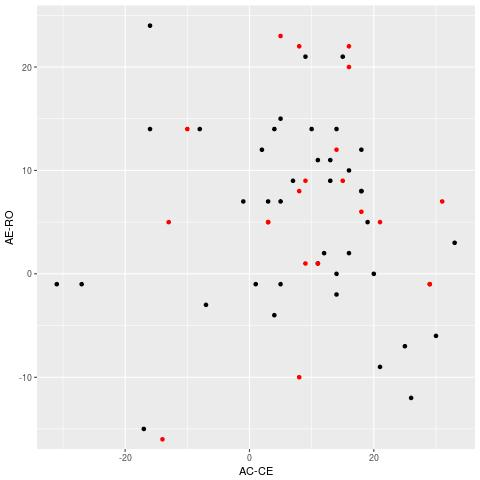
\includegraphics[width=0.7\textwidth]{figures/chapter4/cs-v-it-plot.jpg}
  \caption[AC$-$CE and AE$-$RO for CS and IT Students]{AC$-$CE and AE$-$RO for CS and IT Students}
  \label{fig:cs-v-it-plot}
\end{figure}

Next, I needed to know if the data was normally distributed in order to determine which correlation model to run. To determine if the data was normally distributed, I ran the Shapiro-Wilk test (see Table~\ref{tab:shapiro-wilk} (note that $p<0.05$ here means that the data is \emph{not} normally distributed)). From this analysis, I can see that CS AC$-$CE was the only non-normal data with $p=0.0251$. These findings will be discussed alongside the first research question.

\begin{table}[!htb]
  \centering
  \caption{Shapiro-Wilk Tests}
  \label{tab:shapiro-wilk}
  \begin{tabular}{lll}
    \toprule
    Data         & W       & $p$-value \\
    \midrule
    CS major GPA & 0.95843 & 0.148  \\
    IT major GPA & 0.97703 & 0.8639 \\
    CS AC$-$CE   & 0.93586 & 0.0251 \\
    CS AE$-$RO   & 0.98255 & 0.7826 \\
    IT AC$-$CE   & 0.9529  & 0.3601 \\
    IT AE$-$RO   & 0.95844 & 0.4583 \\
    \bottomrule
  \end{tabular}
\end{table}

\section{Answering the Research Questions}
\subsection{How Strong is the Correlation Between AC$-$CE and AE$-$RO, and Major GPA Among CS, IS, and IT Students?}
Because all of these data points, except for CS AC$-$CE, are normally distributed, I was justified in using Pearson's correlation coefficient (also known as Pearson's $r$) to calculate the correlations. This data is summarized in Table~\ref{tab:pearsons} in which it can be seen that three of the four table entries were not statistically significant, while the IT major GPA and IT AE$-$RO, with $p=0.0202$, was statistically significant.

\begin{table}[!htb]
  \centering
  \caption{Pearson's $r$}
  \label{tab:pearsons}
  \begin{tabular}{lll}
    \toprule
    Data                        & $p$-value & $r$ \\
    \midrule
    CS major GPA and CS AC$-$CE & 0.8177    & -0.0376 \\
    CS major GPA and CS AE$-$RO & 0.6704    & -0.0694 \\
    IT major GPA and IT AC$-$CE & 0.9727    & -0.0077 \\
    IT major GPA and IT AE$-$RO & 0.0202    & 0.4915  \\
    \bottomrule
  \end{tabular}
\end{table}

Since CS students' AC$-$CE results were not normally distributed, I ran Spearman's correlation coefficient to determine if there was a correlation between CS major GPA and CS AC$-$CE results. This resulted in $p>0.05$, but R gave a warning that Spearman's shouldn't be used for data with tied values. To account for the tied values, I then ran the correlation using Kendall's $\tau_b$ which also had $p>0.05$. With Pearson's $r$, Spearman's $\rho$, and Kendall's $\tau_b$ all having $p>0.05$, I am confident that there is no statistically significant correlation between CS major GPA and CS AC$-$CE results.

So, how strong is the correlation between AC$-$CE and AE$-$RO, and major GPA among CS, IS, and IT students? Because of these findings, I am unable to find a statistically significant correlation between any major GPA and a student's LSI results, except for IT major GPA and IT AE$-$RO (see Figure~\ref{fig:major_gpa_lm_plots}). In fact, IT AE$-$RO is so strongly correlated to IT major GPA that it has an $R^2=r^2=0.4915^2=0.2416$. This means that an IT student's AE$-$RO score is able to explain 24.16\% of their GPA. Interestingly, the AC$-$CE spectrum did not hold any statistically significant ($p>0.05$) effect on student GPA in CS or IT. This is interesting because Lunt found that AC$-$CE was the significant axis among electronics students~(Lunt, 1996).

\begin{figure}
  \centering
  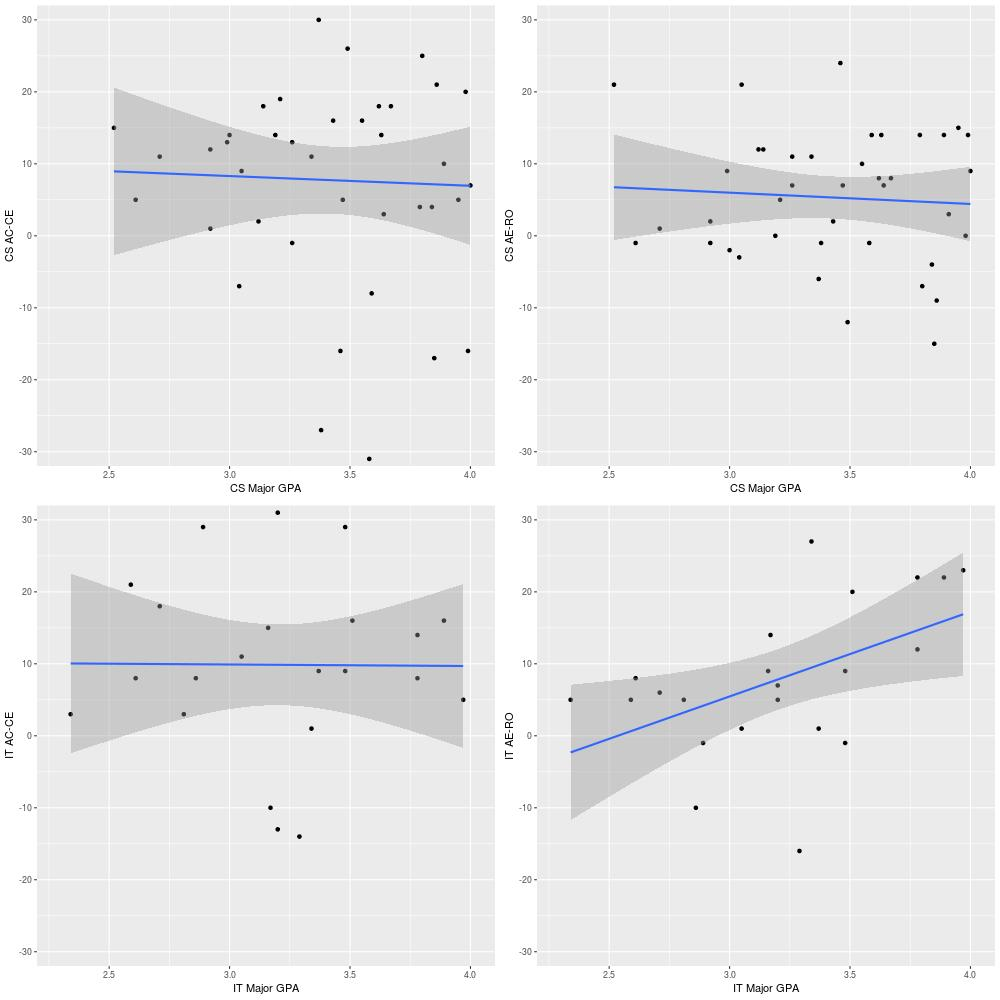
\includegraphics[width=1.1\textwidth]{figures/chapter4/major_gpa_lm_plots.jpg}
  \caption{Correlations Between Major GPA and LSI Results}
  \label{fig:major_gpa_lm_plots}
\end{figure}

\subsection{What is the Best Multiple Regression Model to Fit These Correlations?}
In order to estimate the relationship that AC$-$CE and AE$-$RO each have simultaneously, I developed several multiple regression models. I ran these models with standard errors computed with the Huber-White (HC1) robust standard error to account for the heteroskedasticity of the data. The most significant models can be seen in Table~\ref{tab:mr-models}. All three models used major GPA as the dependent variable, and compared that against the CS dummy variable (to determine if the student is a CS major), age, and parents' education level. Model~2 added AE$-$RO as a covariate, and Model~3 added AC$-$CE as a covariate.

% Table created by stargazer v.5.2 by Marek Hlavac, Harvard University. E-mail: hlavac at fas.harvard.edu
% Date and time: Sun, Jan 28, 2018 - 01:49:51 PM
\begin{table}[!htbp] \centering
  \caption{Multiple Regression Models}
  \label{tab:mr-models}
  \begin{tabular}{@{\extracolsep{5pt}}lccc}
    \toprule
     & \multicolumn{3}{c}{\textit{Dependent variable:}} \\
    \cline{2-4}
    \\[-1.8ex] & \multicolumn{3}{c}{Major GPA} \\
    \\[-1.8ex] & (1) & (2) & (3)\\
    \midrule
    CS dummy variable & 0.110 & 0.137 & 0.137 \\
    &  &  &  \\
    Age 25-29 & $-$0.196 & $-$0.177 & $-$0.177 \\
    &  &  &  \\
    Age 30-34 & $-$0.443 & $-$0.425 & $-$0.426 \\
    &  &  &  \\
    Age 35+ & $-$0.096 & $-$0.077 & $-$0.082 \\
    &  &  &  \\
    Parents education --- & $-$0.661 & $-$0.667 & $-$0.667 \\
    \hspace{2em}some college &  &  &  \\[+0.5em]
    Parents education --- & $-$0.631 & $-$0.534 & $-$0.534 \\
    \hspace{2em}undergraduate degree &  &  &  \\[+0.5em]
    Parents education --- & $-$0.680 & $-$0.602 & $-$0.601 \\
    \hspace{2em}graduate degree &  &  &  \\[+0.5em]
    Parents education --- & $-$0.157 & $-$0.080 & $-$0.080 \\
    \hspace{2em}post-graduate degree &  &  &  \\[+0.5em]
    AE.RO &  & 0.007 & 0.007 \\
    &  &  &  \\
    AC.CE &  &  & 0.0002 \\
    &  &  &  \\
    Constant & 3.976$^{*}$ & 3.828$^{*}$ & 3.826$^{*}$ \\
    & (0.159) & (0.110) & (0.103) \\
    \midrule
    Observations & 62 & 62 & 62 \\
    $R^{2}$ & 0.367 & 0.389 & 0.389 \\
    Adjusted $R^{2}$ & 0.272 & 0.283 & 0.269 \\
    Residual Std. Error & 0.364 (df = 53) & 0.361 (df = 52) & 0.365 (df = 51) \\
    F Statistic & 3.848$^{*}$ (df = 8; 53) & 3.681$^{*}$ (df = 9; 52) & 3.250$^{*}$ (df = 10; 51) \\
    \bottomrule
    \textit{Note:}  & \multicolumn{3}{r}{$^{*}p<0.05$} \\
  \end{tabular}
\end{table}

These models each have statistically significant ($p<0.05$) F statistics, so I reject the null hypothesis that that these groups of variables do not have a statistically significant joint effect. However, an interesting thing happens between models~2 and~3: adding the AC$-$CE covariate decreases the adjusted $R^2$. This means that while the model is still significant with that covariate, it doesn't explain the variance as well. Again, this goes against what Lunt found concerning AC$-$CE results~(Lunt, 1996). Because models~1 and~2 represent the best multiple regression models for this data, I chose to only plot those two (Figure~\ref{fig:mr_models_1_2}).

\begin{figure}[p!]
  \centering
  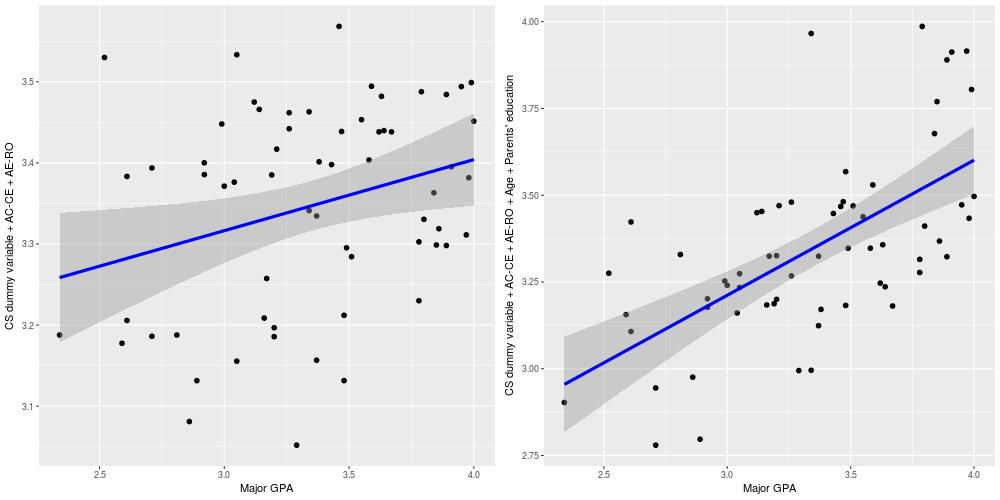
\includegraphics[width=1.1\textwidth]{figures/chapter4/mr_models_1_2.jpg}
  \caption{Multiple Regression Models 1 and 2}
  \label{fig:mr_models_1_2}
\end{figure}

Up to this point, I've only examined individual variables, not groups of variables. The linear hypothesis test compares the residual (error) sum of squares values against similar models. This way, I can check individual variables for a joint significance which will allow me to see if the variables can explain the deviance in the model. The null hypothesis is that each of these variables are 0. This test is important because removing unnecessary variables gives more power with this small of a dataset.

The model I ran used major GPA as the dependent variable, and compared it to the CS dummy variable, AE$-$RO, age, and parents education. This model had $p=1.266\times 10^{-10}$, so I reject the null hypothesis that at least one of these variables is not significant in explaining the variance in the data. This model reinforces the earlier, multiple regression findings.

\subsection{How Strong is the Correlation Between AC$-$CE and AE$-$RO, and Student Satisfaction Among CS, IS, and IT Students?}
Nuata's AMSS, as enumerated in chapter 1, is graded on a five-point Likert-type scale with two of the responses being negatively scored. Two of the AMSS questions assume that students still have the option of changing their major, but once BYU students get beyond a certain credit threshold (well before their senior year), it becomes impossible for them to change majors. Because of this and the lack of variance among the responses, these questions were dropped from the analysis:
\begin{enumerate}
  \item I am strongly considering changing to another major.
  \item I would like to talk to someone about changing my major.
\end{enumerate}

I created a summary index of academic major satisfaction using the remaining AMSS variables and reverse coded the negatively-scored variables. In this summary index, the least satisfied value was a 4 and the most satisfied was a 20, with a mean of $18.10$ ($\sigma=2.2595$). This data is heavily left-skewed (see Figure~\ref{fig:amss_index_plot}).

\begin{figure}[p]
  \centering
  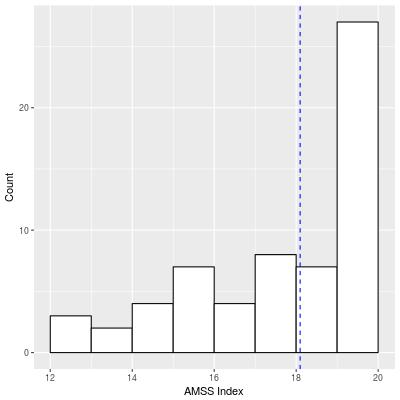
\includegraphics[width=0.85\textwidth]{figures/chapter4/amss_index_plot.jpg}
  \caption{AMSS Index Histogram}
  \label{fig:amss_index_plot}
\end{figure}

I then ran a linear regression model for the data and found no statistically significant results (see Table~\ref{tab:amss_corr}), suggesting that there is no relationship between learning style and major satisfaction. I believe the lack of response diversity led, at least in part, to the lack of correlations between student satisfaction and learning style.

% Table created by stargazer v.5.2 by Marek Hlavac, Harvard University. E-mail: hlavac at fas.harvard.edu
% Date and time: Sat, Feb 17, 2018 - 05:00:22 PM
\begin{table}[p]
  \centering
  \vspace{0.5in}
  \caption{AMSS Correlations}
  \label{tab:amss_corr}
  \begin{tabular}{@{\extracolsep{5pt}}lcc}
    \toprule
    & \multicolumn{2}{c}{\textit{Dependent variable:}} \\
    \cline{2-3}
    \\[-1.8ex] & CS AMSS Index & IT AMSS Index \\
    \midrule
    CS AC$-$CE & 0.011 &  \\
    & & \\
    CS AE$-$RO & 0.066 &  \\
    & & \\
    IT AC$-$CE &  & $-$0.003 \\
    & & \\
    IT AE$-$RO &  & 0.029 \\
    & & \\
    Constant & 17.665$^{*}$ & 17.890$^{*}$ \\
    & (0.528) & (0.022) \\
    & & \\
    \hline \\[-1.8ex]
    Observations & 40 & 22 \\
    $R^{2}$ & 0.065 & 0.022 \\
    Adjusted $R^{2}$ & 0.015 & $-$0.081 \\
    Residual Std. Error & 2.344 (df = 37) & 2.198 (df = 19) \\
    F Statistic & 1.294 (df = 2; 37) & 0.212 (df = 2; 19) \\
    \bottomrule
    \textit{Note:}  & \multicolumn{2}{r}{$^{*}$p$<$0.05} \\
  \end{tabular}
  \newline
  \vspace{0.5in}
\end{table}

\subsection{Is There a Correlation Between Major GPA and Student Satisfaction?}
To determine if there was a correlation between major GPA and student satisfaction, I ran a linear regression model against the data (Table~\ref{tab:satisfaction} and Figure~\ref{fig:major_gpa_amss_plots}), with major GPA being the dependent variable and each major's AMSS index as the independent variables.

% Table created by stargazer v.5.2 by Marek Hlavac, Harvard University. E-mail: hlavac at fas.harvard.edu
% Date and time: Tue, Feb 20, 2018 - 08:41:03
\begin{table}[!htbp]
  \centering
  \vspace{1in}
  \caption{Major GPA and Student Satisfaction}
  \label{tab:satisfaction}
  \begin{tabular}{@{\extracolsep{5pt}}lcc}
    \toprule
     & \multicolumn{2}{c}{\textit{Dependent variable:}} \\
    \cline{2-3}
    \\[-1.8ex] & CS Major GPA & IT Major GPA \\
    \\[-1.8ex] & (1) & (2)\\
    \midrule
     CS AMSS index & 0.028 &  \\
      & & \\
     IT AMSS index &  & 0.035 \\
      & & \\
     Constant & 2.919$^{*}$ & 2.563$^{*}$ \\
      & (0.513) & (0.028) \\
      & & \\
    \midrule
    Observations & 40 & 22 \\
    $R^{2}$ & 0.027 & 0.028 \\
    Adjusted $R^{2}$ & 0.002 & $-$0.020 \\
    Residual Std. Error & 0.401 (df = 38) & 0.448 (df = 20) \\
    F Statistic & 1.062 (df = 1; 38) & 0.585 (df = 1; 20) \\
    \bottomrule
    \textit{Note:}  & \multicolumn{2}{r}{$^{*}$p$<$0.05} \\
  \end{tabular}
  \newline
  \vspace{1in}
\end{table}

\begin{figure}[!hbtp]
  \centering
  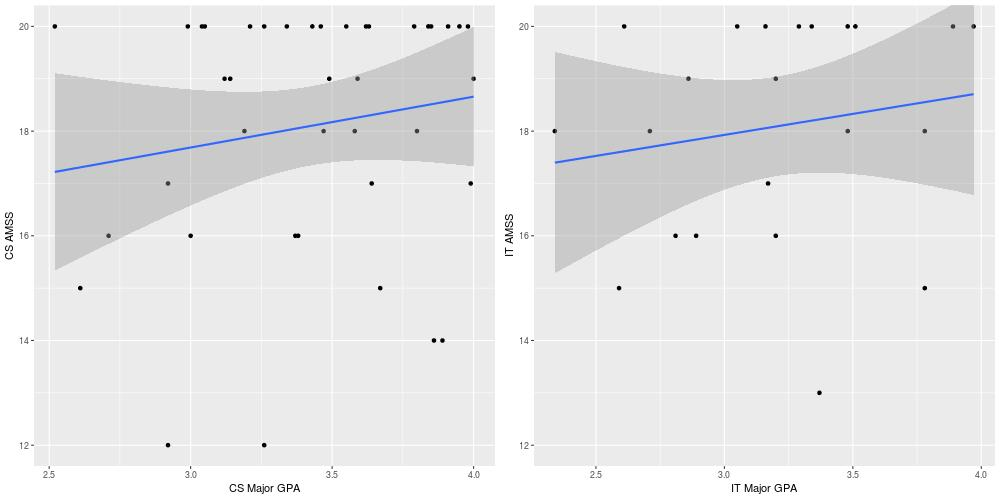
\includegraphics[width=1.05\textwidth]{figures/chapter4/major_gpa_amss_plots.jpg}
  \caption{Major GPA and Student Satisfaction Correlations}
  \label{fig:major_gpa_amss_plots}
\end{figure}

This regression model had $p>0.05$, so I am unable to say that there is a significant correlation between the major GPA and student satisfaction.

\section{Demographics}
Unfortunately, I was unable to use the full set of demographic variables collected from students as covariates because there was not enough variance among the sample group. The students were almost entirely white and male (88\% for both). Looking at the relationship between marital status and its effect on major GPA and satisfaction had a multiple $R^2$ of $0.07$, meaning that marital status was only able to explain 7\% of the variance in major GPA and satisfaction. While students were equally divided in marital status (31 single, 31 married), there was no relationship between marital status and any other factor. The multiple regression analysis for the demographic information, calculated with robust standard error, is summarized in Table~\ref{tab:demographics}.

% Table created by stargazer v.5.2 by Marek Hlavac, Harvard University. E-mail: hlavac at fas.harvard.edu
% Date and time: Sun, Jan 28, 2018 - 05:36:26 PM
\begin{table}[!htbp] \centering
  \caption{Demographic Regression Analysis}
  \label{tab:demographics}
  \begin{tabular}{@{\extracolsep{5pt}}lc}
    \toprule
     & \multicolumn{1}{c}{\textit{Dependent variable:}} \\
    \cline{2-2}
    \\[-1.8ex] & AMSS index \\
    \midrule
    Major GPA & 1.088 \\
    &  \\
    CS dummy variable & $-$0.276 \\
    &  \\
    Age 25-29 & $-$0.536 \\
    &  \\
    Age 30-34 & $-$0.034 \\
    &  \\
    Age 35+ & 0.723 \\
    &  \\
    Gender~--- female & $-$3.251 \\
    &  \\
    Gender~--- male & $-$3.275 \\
    &  \\
    Constant & 18.072$^{*}$ \\
    & (2.230) \\
    \midrule
    Observations & 62 \\
    $R^{2}$ & 0.070 \\
    Adjusted $R^{2}$ & $-$0.051 \\
    Residual Std. Error & 2.316 (df = 54) \\
    F Statistic & 0.578 (df = 7; 54) \\
    \bottomrule
    \textit{Note:}  & \multicolumn{1}{r}{$^{*}p<0.05$} \\
  \end{tabular}
\end{table}
